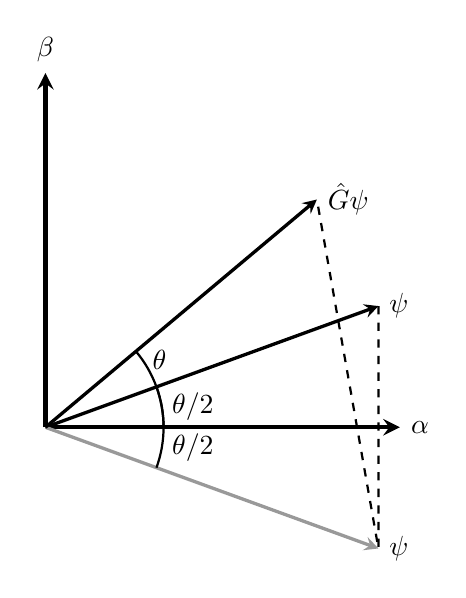
\begin{tikzpicture}
  [scale=1.5,
  axis/.style={ultra thick,->,>=stealth},
  vec/.style={very thick,->,>=stealth},
  angles/.style={thick}]

  % define the angle theta in terms units of degrees
  \def\ang{20}

  % origo
  \coordinate (O) at (0,0);

  % draw axis
  \draw[axis] (O) -- (3,0) node [anchor=west]   {$\ket{\alpha}$};

  \draw[axis] (O) -- (0,3) node [anchor=south]  {$\ket{\beta}$};

  % vectors
  \draw[vec]          (O) -- (\ang:3cm) node [right]
  {$\ket{\psi}$};

  \draw[vec,black!40] (O) -- (-\ang:3cm) node [right,text=black]
  {$\operator\ket{\psi}$};

  \draw[vec]          (O) -- ({2*\ang}:3cm) node [right]
  {$\hat{G}\ket{\psi}$};

  % draw lines connecting the vectors
  \draw[dashed,thick] (\ang:3cm) -- (-\ang:3cm) -- ({2*\ang}:3cm);

  % draw angles
  \draw[angles] (1,0) arc [start angle=0, end angle=\ang, radius=1]
  node[midway, right] {$\theta/2$};

  \draw[angles] (1,0) arc [start angle=0, end angle=-\ang, radius=1]
  node[midway, right] {$\theta/2$};

  \draw[angles] (1,0) arc [start angle=0, end angle={2*\ang}, radius=1]
  node[very near end, right] {$\theta$};
\end{tikzpicture}
